\chapter{Criticallink MitySOM SoC}
Altera was founded in 1983 and developed their first FPGA in 1992.\cite{althist16} The Altera Cyclone V was developed to decrease time-to-market and cost requirements, simultaneously the power consumption is decreased. Cyclone V devices are made in 28nm technology and have a core volage of 1.1V. The 10kB memory blocks have a built in soft ECC. \cite{altcycvov15}
\begin{figure}[htbp]
\begin{center}
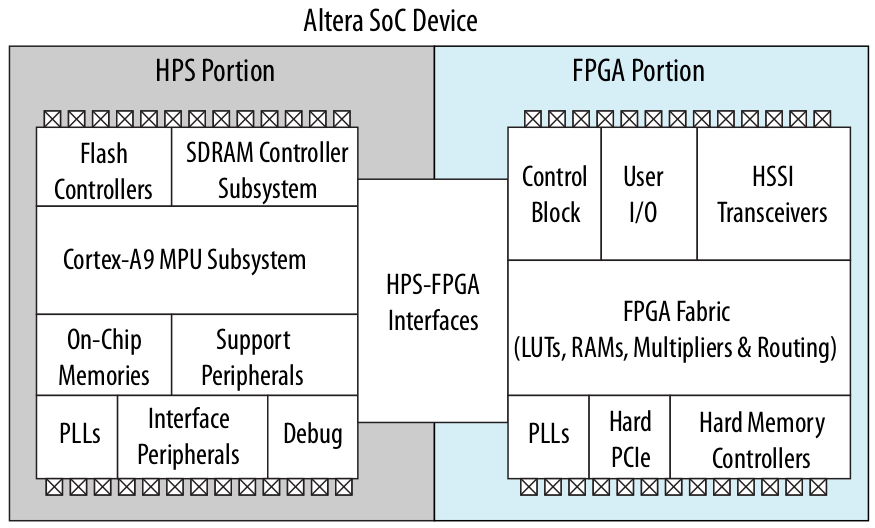
\includegraphics[width=10cm,keepaspectratio=true]{bilder/png/AlteraSoC}
\caption{Block diagram of an Altera Cyclone V SoC\cite[chapter 1]{AlteraHPS15}}
\label{fig:alterasocblocks}
\end{center}
\end{figure}
\section{FPGA}
\section{HPS}
\begin{figure}[htbp]
\begin{center}
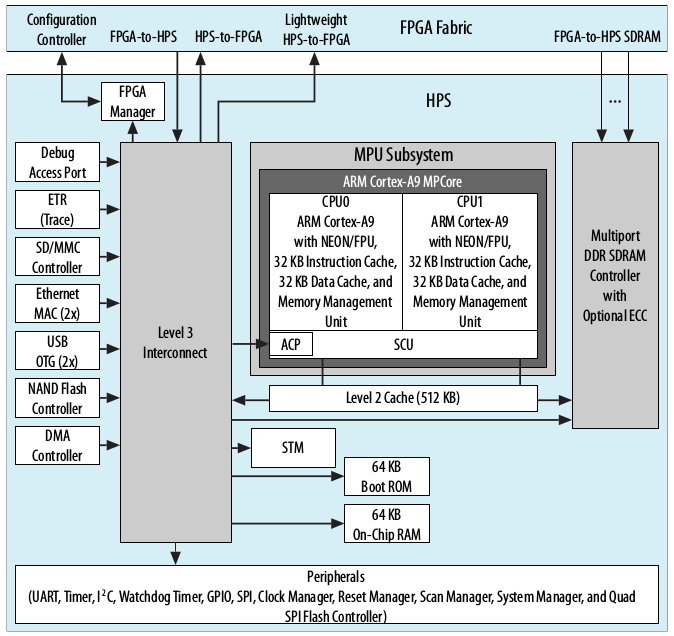
\includegraphics[width=15cm,keepaspectratio=true]{bilder/png/AlteraHPSneu}
\caption{Block diagram of an Altera Cyclone V HPSneu\cite{altcycvov15}}
\label{fig:alterahpsblocksneu}
\end{center}
\end{figure}
\begin{figure}[htbp]
\begin{center}
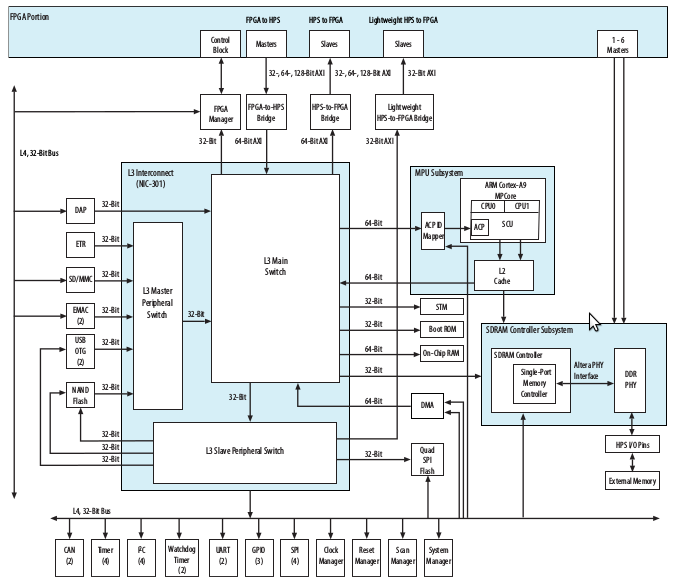
\includegraphics[width=15cm,keepaspectratio=true]{bilder/png/AlteraHPS}
\caption{Block diagram of an Altera Cyclone V HPS\cite[chapter 1]{AlteraHPS15}}
\label{fig:alterahpsblocks}
\end{center}
\end{figure}
\section{FPGA-HPS-Bridge}
\section{Interfaces}
\subsection{UART}
\subsection{GPIO}
\subsection{I$^2$C}
The I$^2$C-bus was intentionally developed by Philips in the early 1980s to exchange information between ICs located on the same board. This bus is designed for synchronous transmission and is built up of ground, data and clock line. As advantage of this protocol the clock reconstruction possibilities at the receiver has to be mentioned. Furthermore an arbitrary protocol guarantees that only one master exists at one time.\cite{Wue06} I$^2$C defines communication modes as follows:
\begin{table}
\begin{center}
\begin{tabular}{|c||c|c|}
\hline
mode & maximum transmission speed & direction\\
\hline\hline
standard mode & 100 kbit/s & bidirectional\\
\hline
full speed & 400 kbit/s & bidirectional\\
\hline
fast mode & 1 Mbit/s & bidirectional\\
\hline
high speed mode & 3.2 Mbit/s & bidirectional\\
\hline
ultra fast mode (UFm) & 5 Mbit/s & unidirectional\\
\hline
\end{tabular}
\caption{Speed grades of I$^2$C-transmissions\cite{I2Cspeed}}
\label{tab:rsstates}
\end{center}
\end{table}
As the I$^2$C-bus is inteded to exchange data between ICs the packet size is small. This leads to the fact that high accuracy of the clock is not needed for most applications.\cite{I2Cspeed} Intentionally the I$^2$C-bus was designed for 5V reference voltage. With the release of the specification I$^2$C-2.0 the bus got also the possibility to operate with 2V references.\cite{I2Cvoltage}
More information can be found in the I$^2$C-specification in \cite{I2Cspec}.
\subsection{CAN}
The CAN-bus was developed by Bosch in the early 1980s as serial communication protocol for motorized vehicles. In 1994 it became an international standard ISO 11898. The protocol is able to handle bitrates up to 1 Mbit/s and has multi-master capability. That means that different bus members can have master state at different times. CAN is able to handle reference voltages of 5V and 3.3V.\cite{Corrig2008} The CAN-bus uses two signaling lines for communications. As CAN is designed as real time control protocol with a high level of security, it has some important features beside others\cite{boschcan91}:
\begin{itemize}
\item message priorization
\item guaranteed latency times
\item different error detection capabilities
\item autonomous switching off of defect nodes
\end{itemize}
The specification of CAN can be found in \cite{boschcan91}, an even more detailed description in \cite{nxpcan98}.